\section{Methods}
\label{sec:methods}

To compute the coarse matrix $Ac$, a triple matrix multiplication should be done:
\begin{equation}
 Ac = R \times A \times P
\end{equation}
in which $R = P^T$.

This section includes two parts: We first explain how the communication is being done between processors. Then, assuming we have the required data, we describe doing the multiplication locallly on one processor.

\subsection{Communication}
\label{sec:comm}

Matrices are partitioned on multiple processors by row blocks (Figure~\ref{fig:partition}). Matrices $A$ and $P$ have the same number of rows and consequently are partitioned the same way. $R$ has less number of rows and has a different partition.

\begin{figure}[tbh]
 \centering
 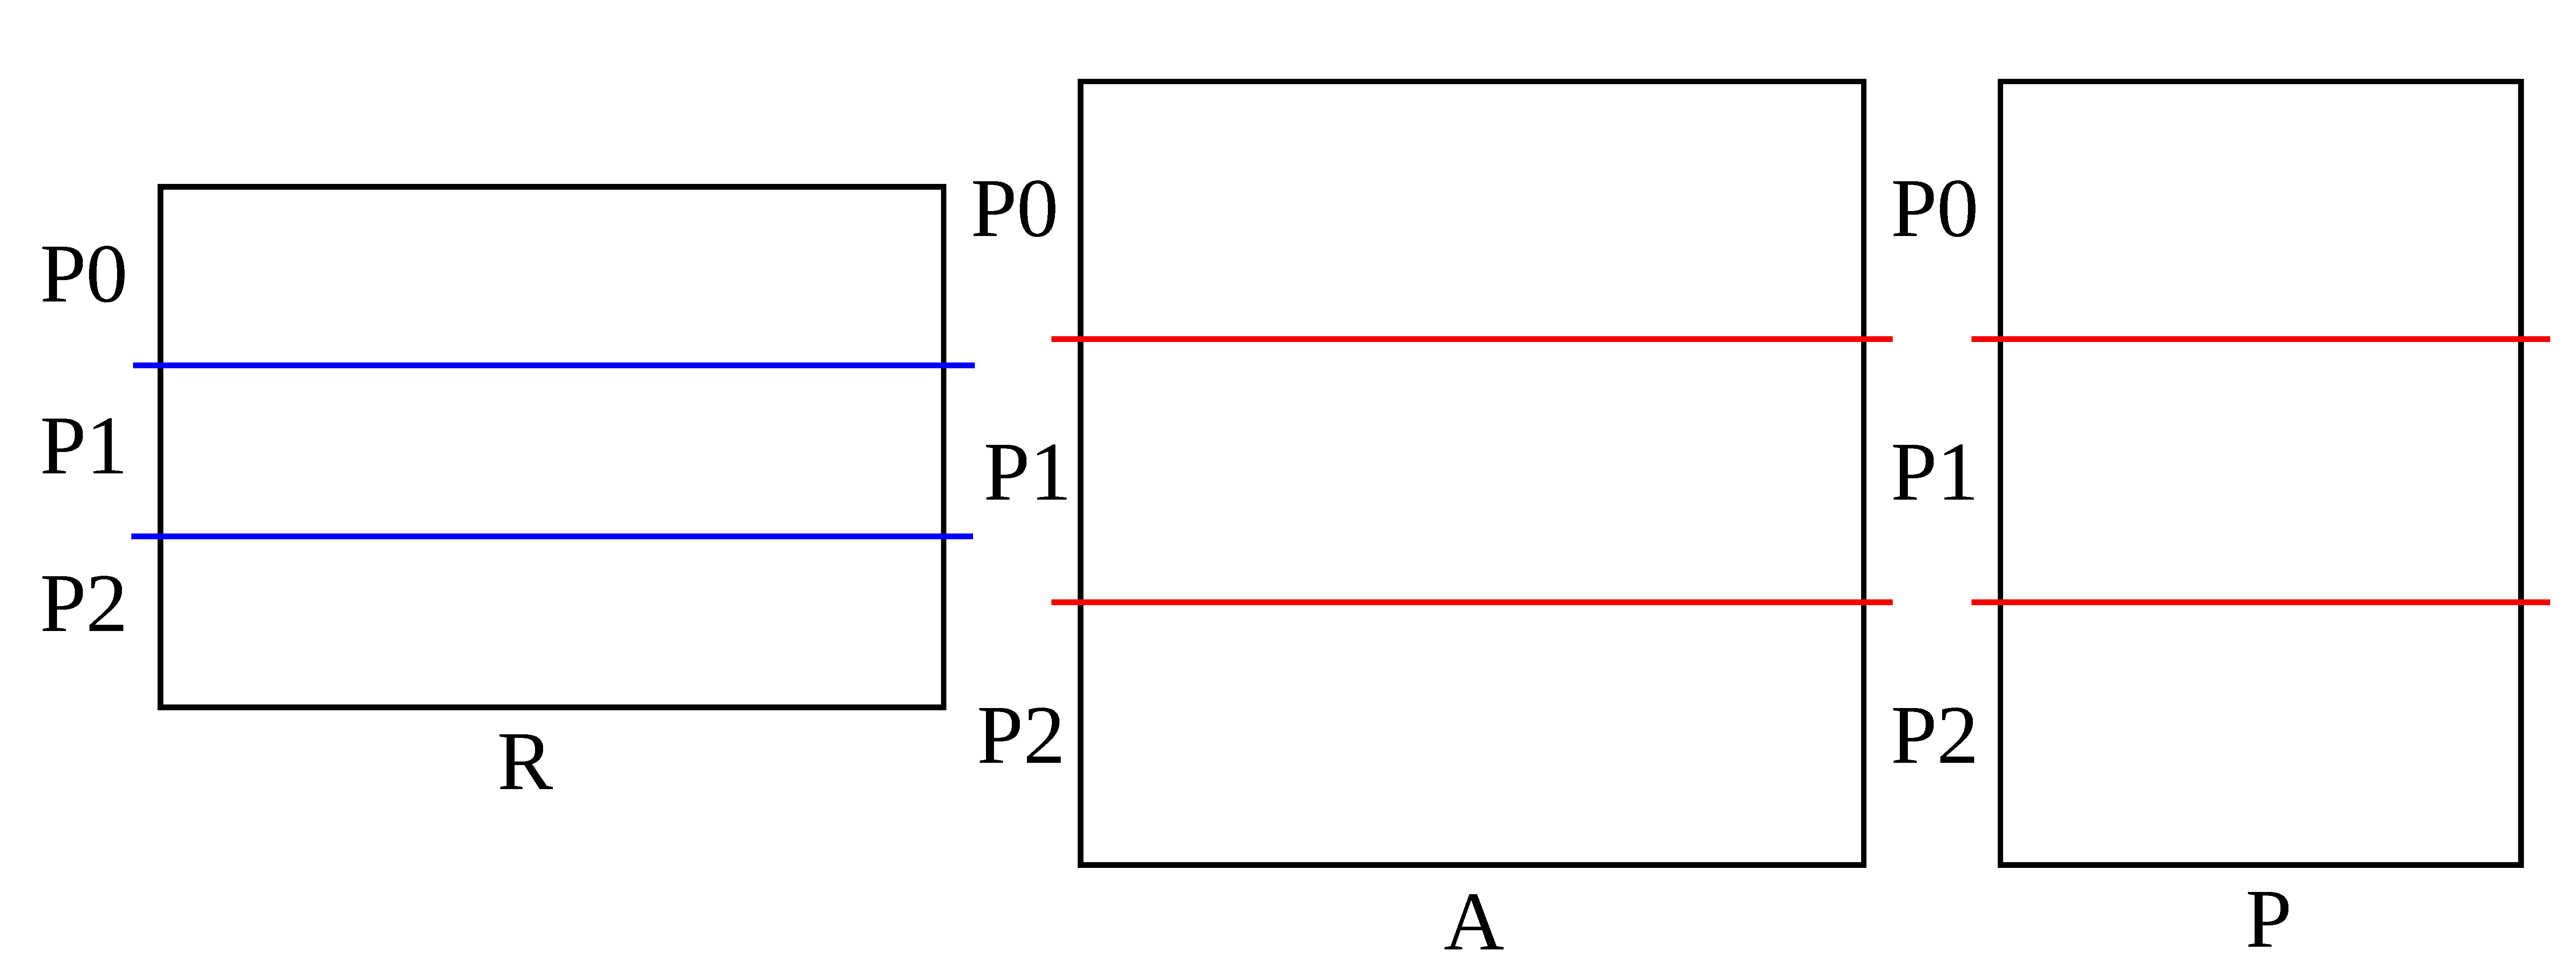
\includegraphics[width=8cm,height=3cm]{./figures/partition.pdf}
 \caption{}
 \label{fig:partition}
\end{figure}

The triple matrix product is being done in two parts: first $A \times P$, then $R \times B$, in which $B = A \times P$, so performing matrix-matrix multiplications (\mm~) twice.

\subsubsection{Part 1}

In this part, we compute $B := A \times P$. We assume the same partition of rows of $A$ on its columns. The same partition of rows of $R$ is assumed on columns of $P$ (Figure~\ref{fig:part1b}).
Here we consider doing \mm ~on processor $P1$. To compute entry $B(i, j)$, we need to multiply row $i$ of $A$ with column $j$ of $P$ and add them together (since we are working with sparse matrices, we only consider the nonzeros).

\begin{figure}[tbh]
 \centering
 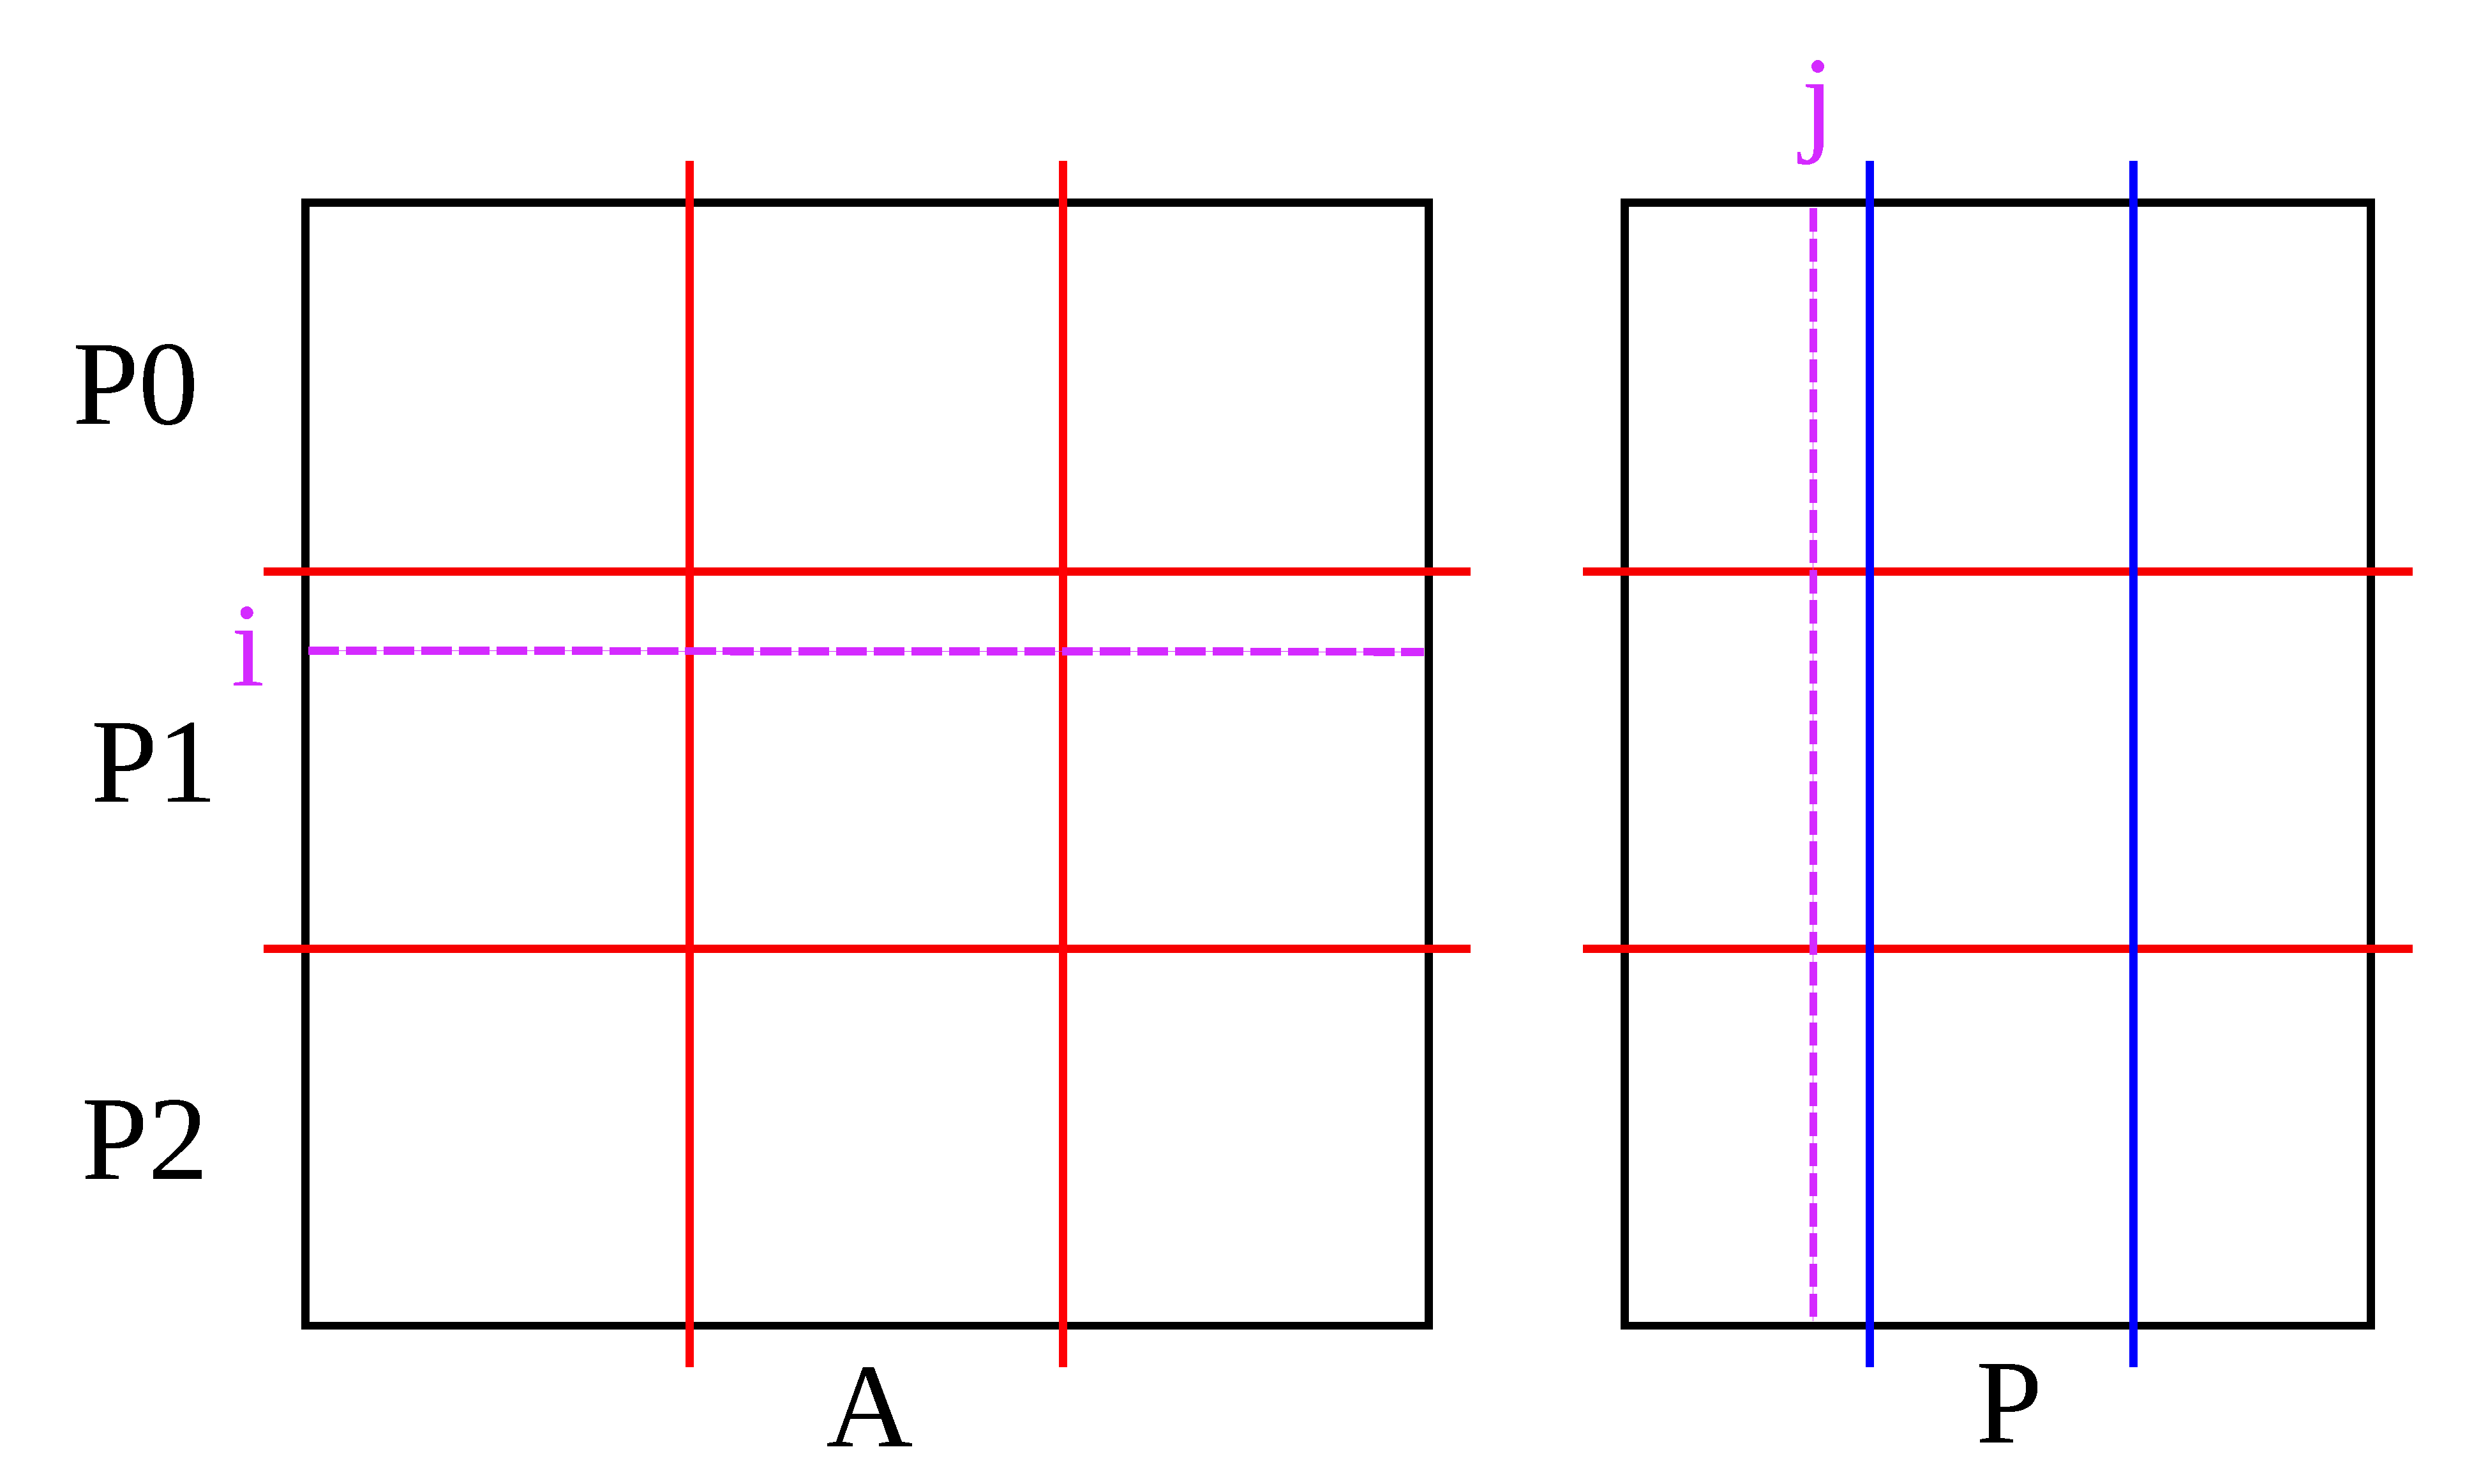
\includegraphics[width=5.5cm,height=3cm]{./figures/part1b.pdf}
 \caption{}
 \label{fig:part1b}
\end{figure}

Column $j$ is distributed between all the processors, so we will be able to perform  summation $B_{ij} = \sum_{k} A_{ik} P_{kj}$, after communicating all nonzeros of column $j$ and performing the multiplication. (explain this part clearer and show why this method is not good). To avoid that, we can use the fact that $R$ is the transpose of $P$ and we already have computed it. We note that column blocks of $P$ (e.g. $r0$ in Figure~\ref{fig:part1c}) are actually row blocks of $R$ transposed ($rt0$, which is transpose of $r0$).

\begin{figure}[tbh]
 \centering
 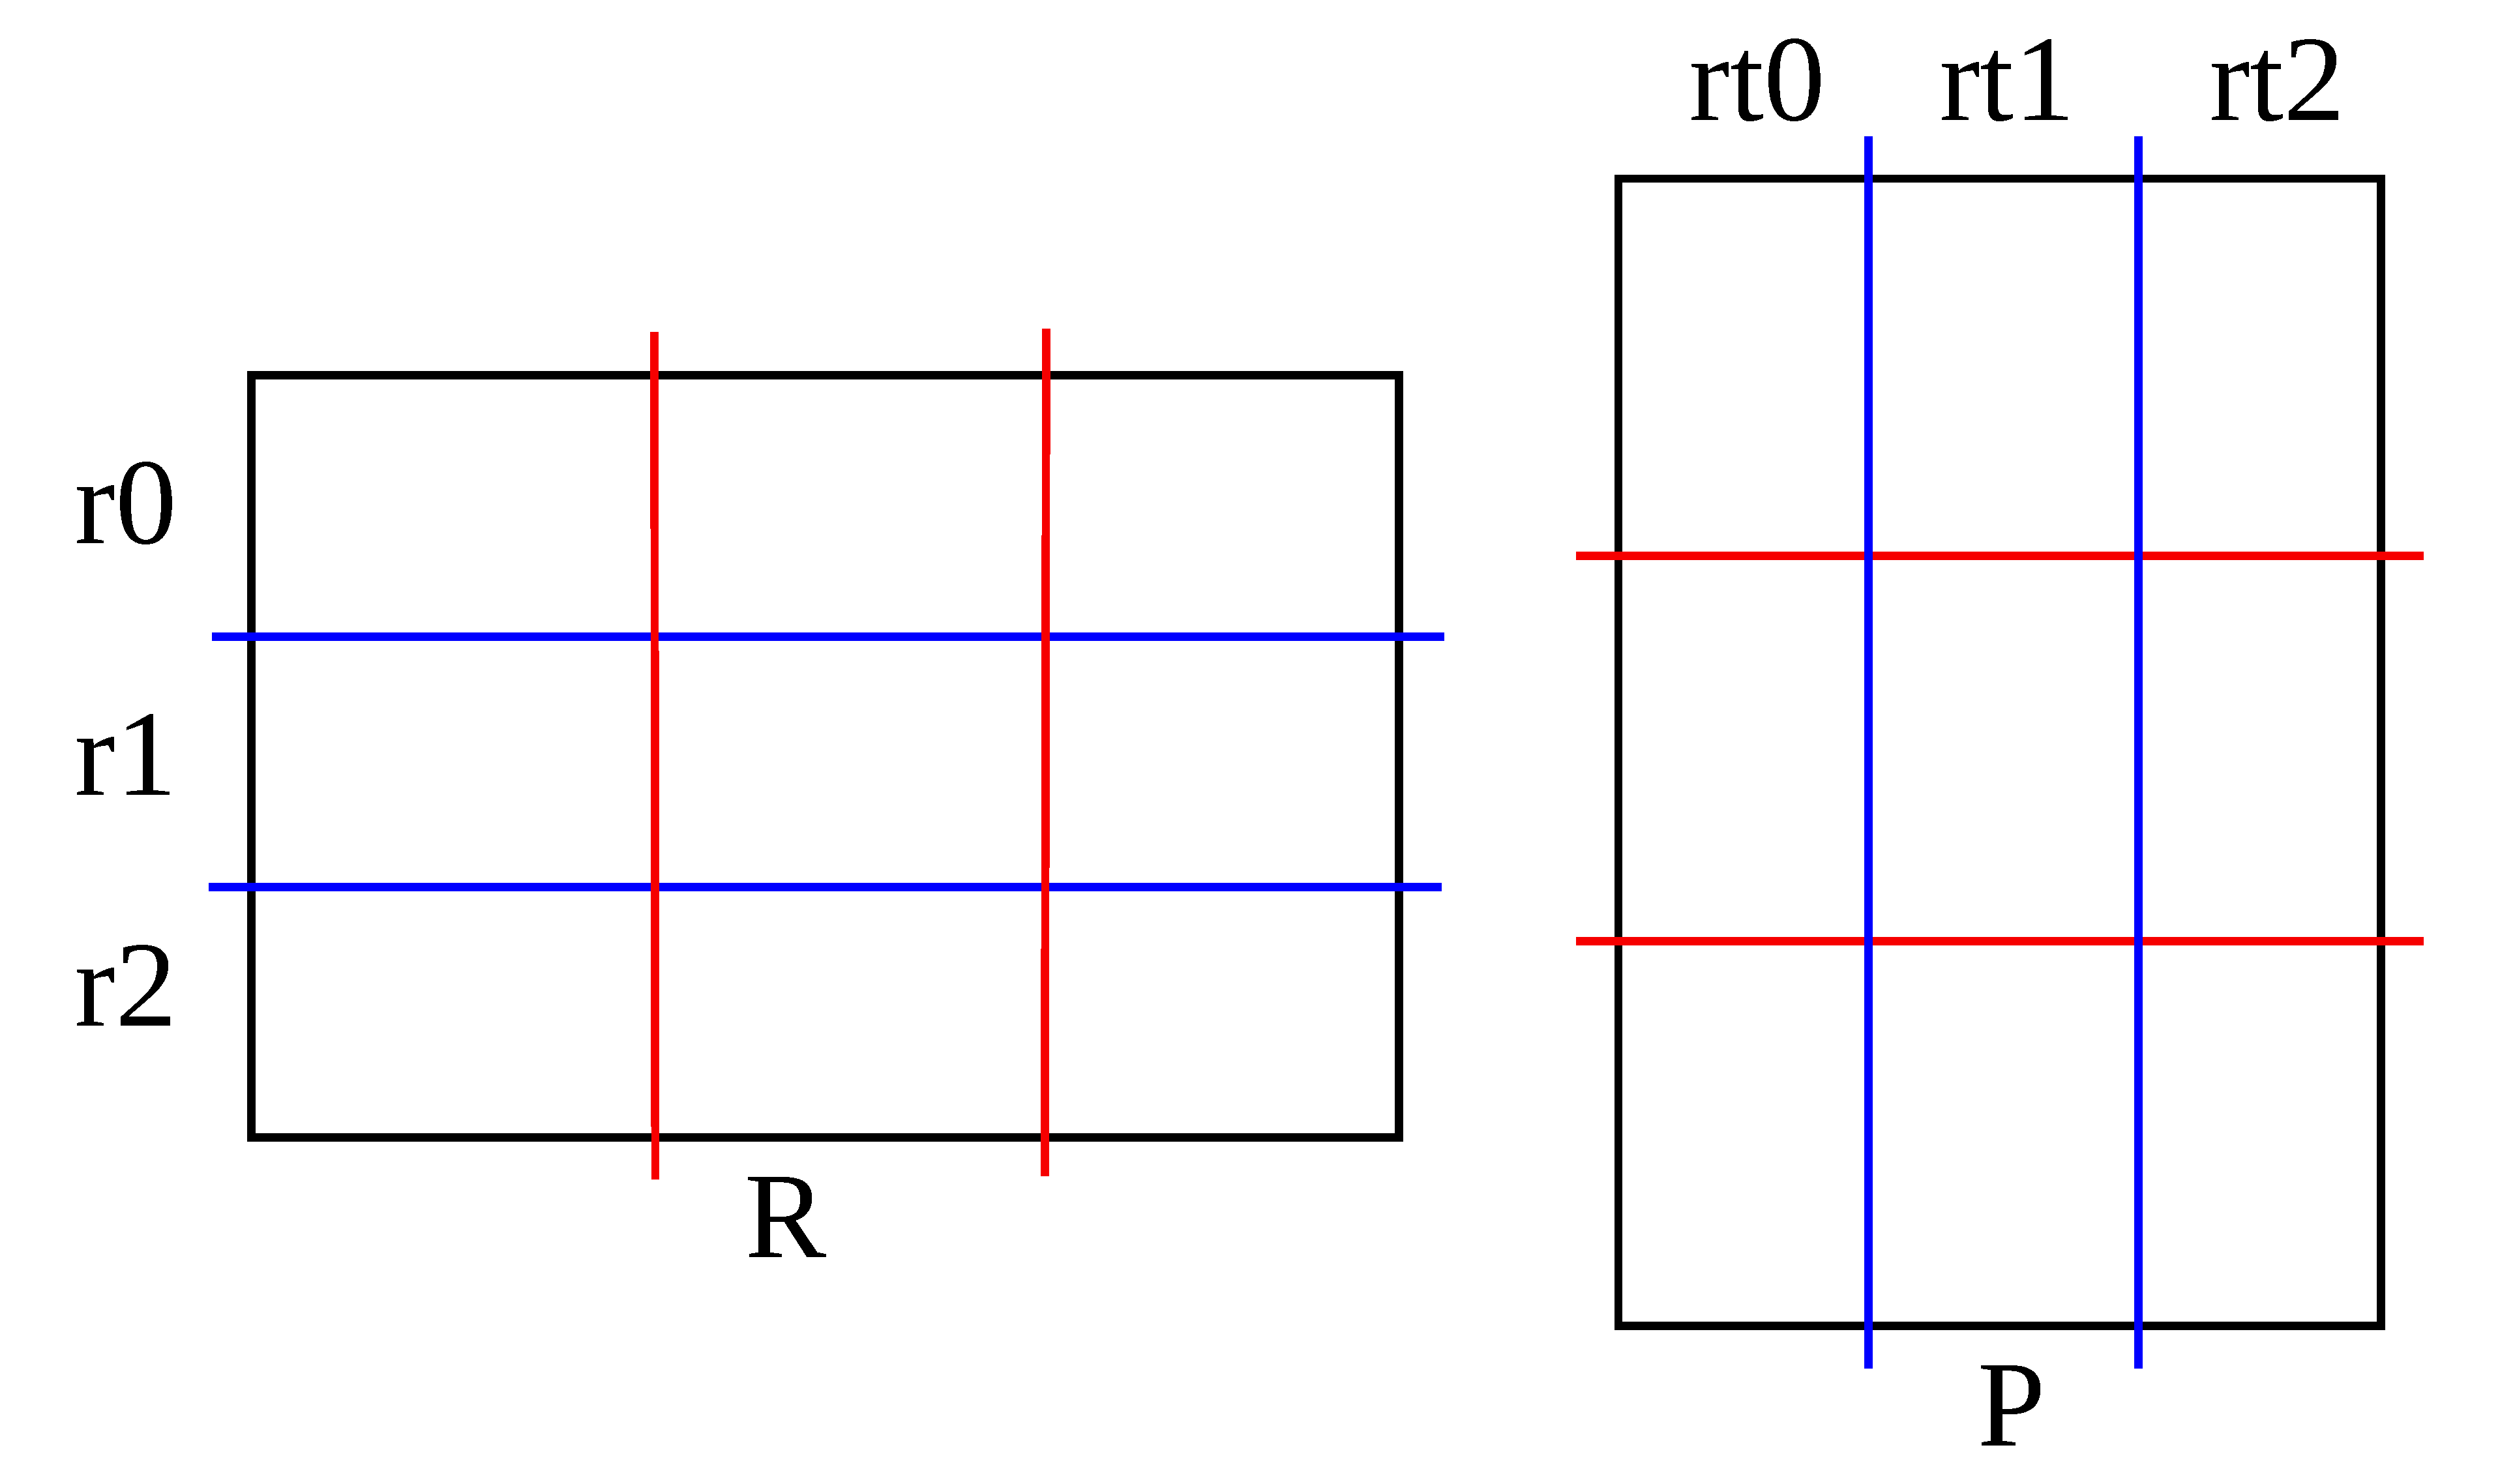
\includegraphics[width=5.5cm,height=3cm]{./figures/part1c.pdf}
 \caption{}
 \label{fig:part1c}
\end{figure}

Algorithm \ref{alg:part1} shows how we do it in an overlapped fashion using MPI. $B_{i}$ is the row block of matrix $B$ on processor $i$ and $B_{ik}$ is the sub-block result of multiplying $A_i$ with $rt_i$.

\begin{algorithm}[H] 
  %\footnotesize
  \caption{Part 1: $B_i = A_i \times P$} \label{alg:part1} 
  \begin{algorithmic}[1]
    \Require $A_i$, $R$
    \Ensure  $B_i$ (result of $A_i \times P$)
    \State $R1 \leftarrow$ compute transpose of $R_i$ (locally)
    \For{$k=myrank:myrank+nprocs$}
      \State $R2 \leftarrow\ Irecv\ transpose\ of\ R\ from\ right\ neighbor$
      \State $Isend(R1)\ to\ left\ neighbor$
      \State $B_{ik} \leftarrow A_i \times R1$
      \State $wait\ for\ Isend\ and\ Irecv\ to\ finish$
      \State $swap(R1,R2)$
    \EndFor
  \end{algorithmic}
\end{algorithm}


\subsubsection{Part 2}

Now we explain how to do the second \mm: $R \times B$, in which $B = A \times P$. Figure~\ref{fig:part2d} shows an example on processor $P1$. The blocks of $R$ on processor $P1$ should be multiplied with the corresponding blocks of $B$ with the same color. To do that we need to communicate whole $B$ between all the processors.

\begin{figure}[tbh]
 \centering
 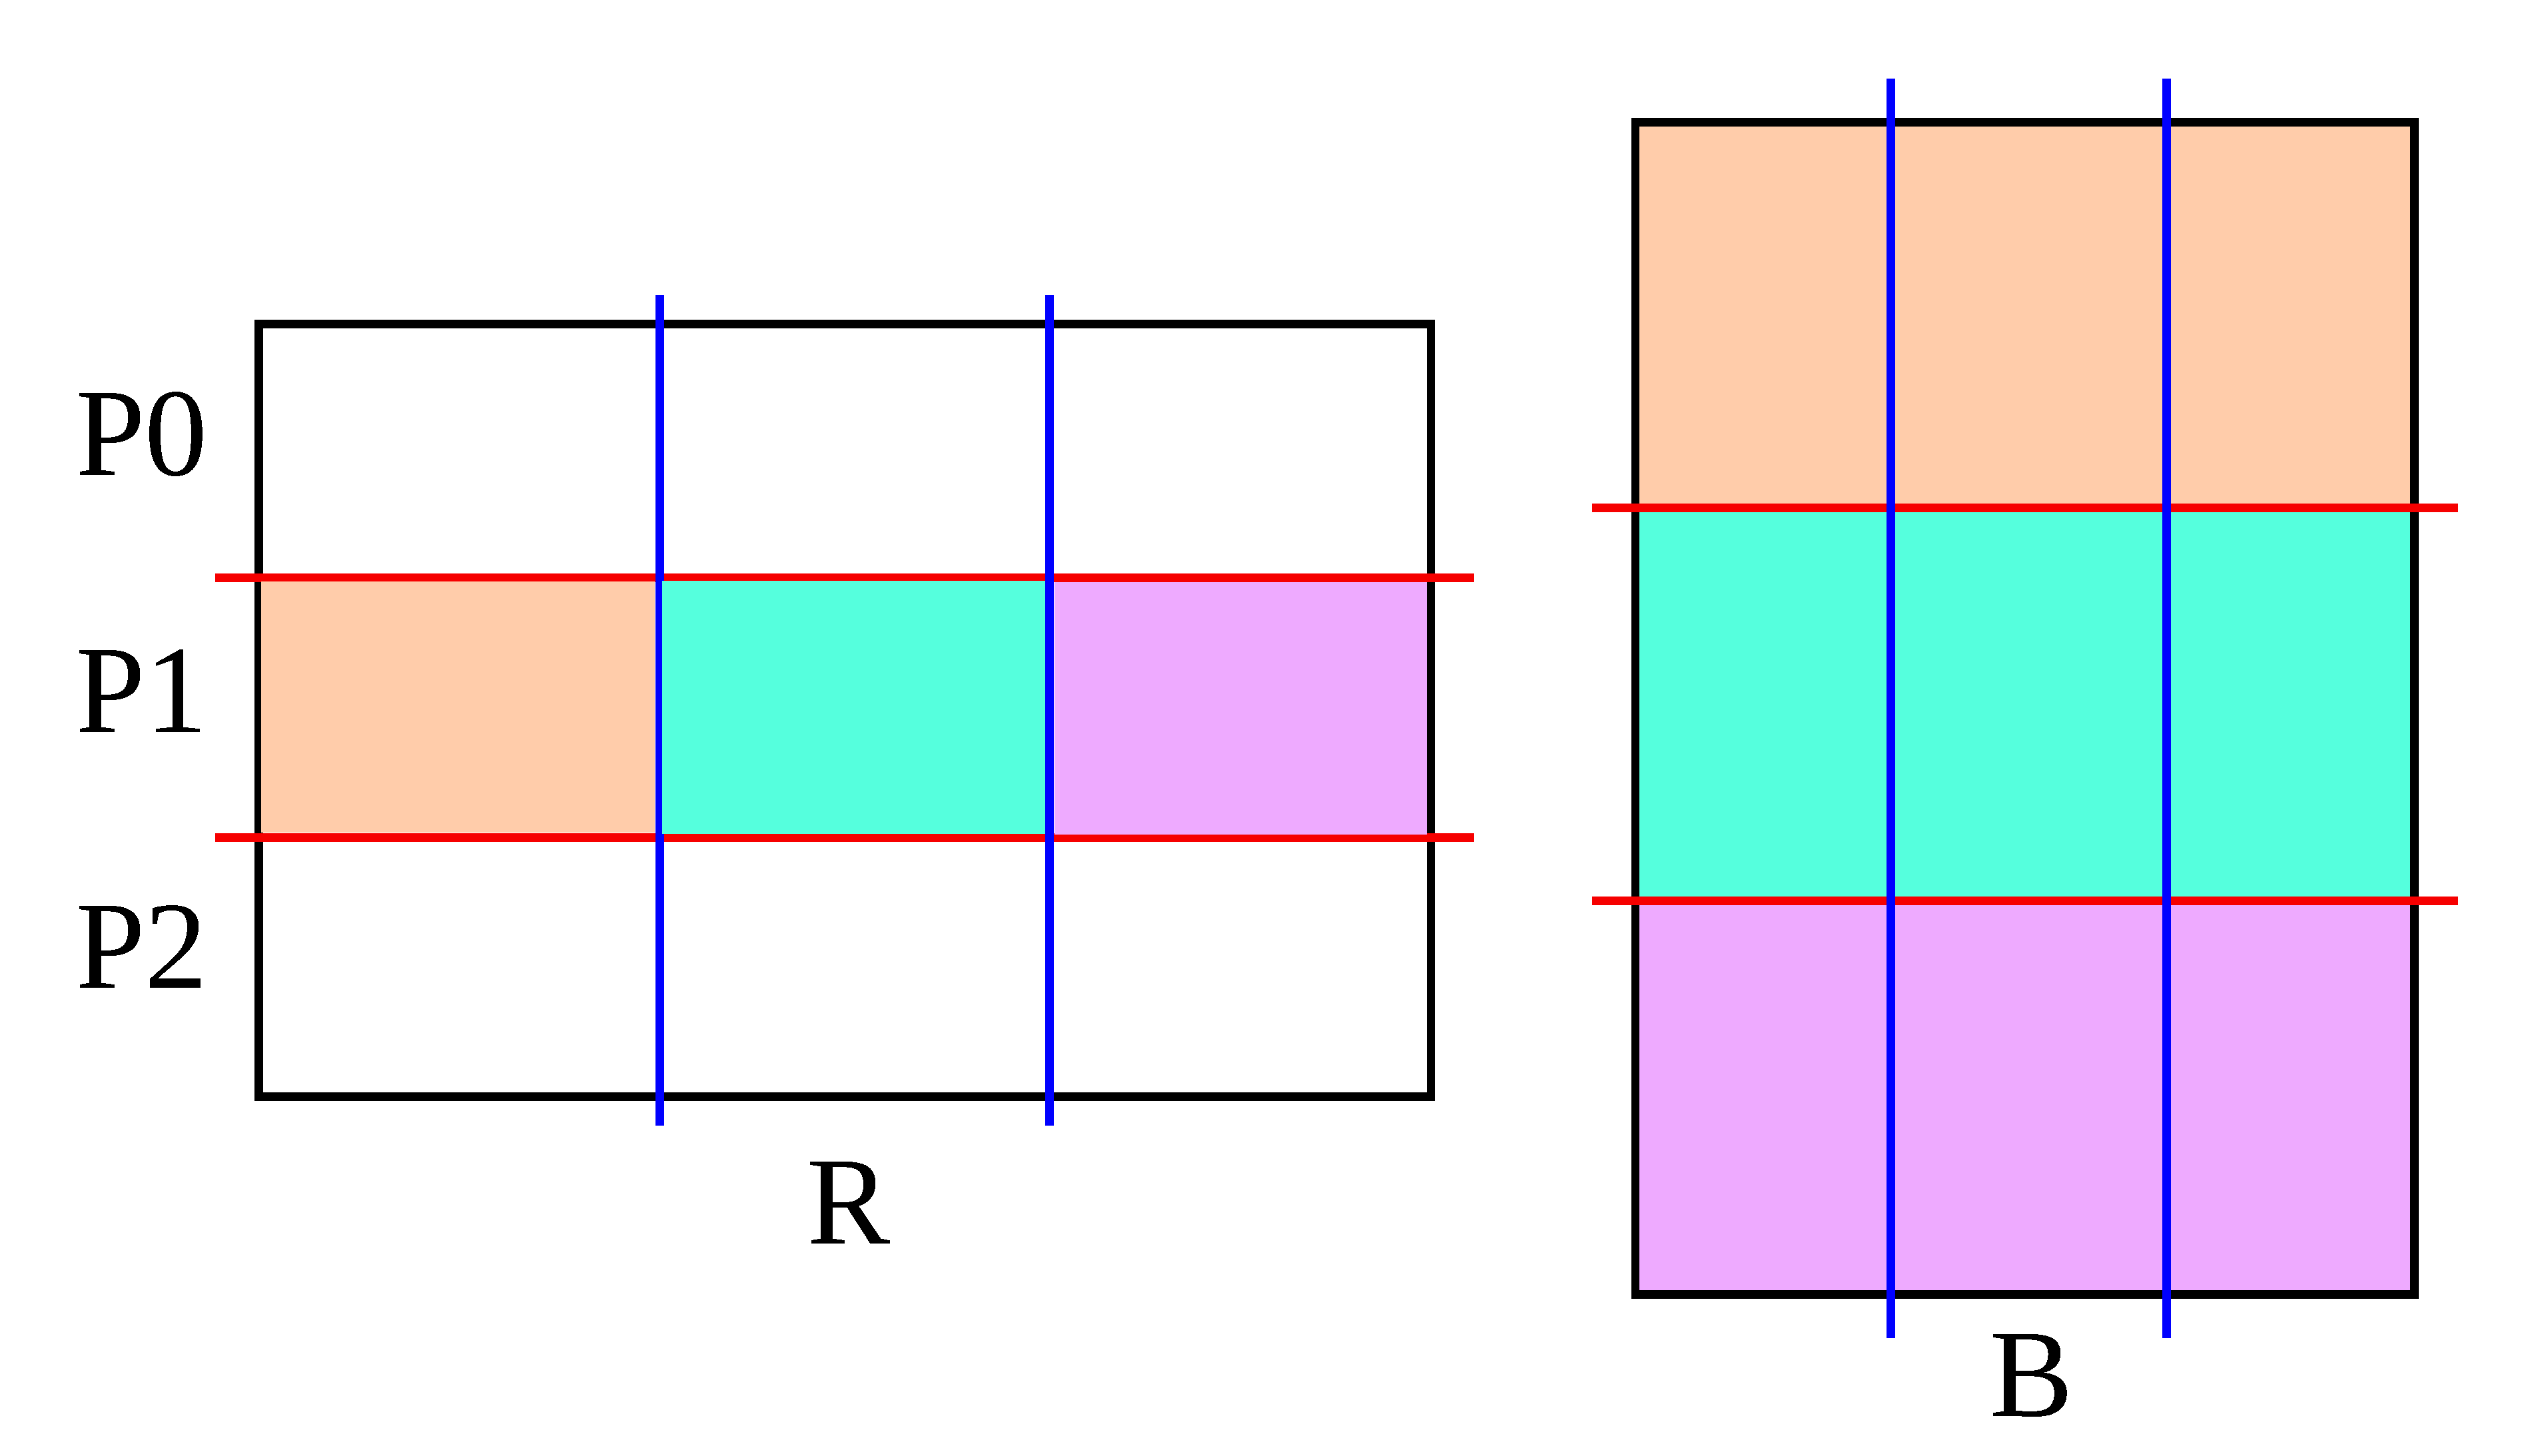
\includegraphics[width=5.5cm,height=3cm]{./figures/part2d.pdf}
 \caption{}
 \label{fig:part2d}
\end{figure}

To avoid this expensive communication, we again can use the fact that we already have computed the transpose of $R$. We only perform the multplication of the green blocks on processor $P1$ in Figure~\ref{fig:part2e}, which can be done locally.

\begin{figure}[tbh]
 \centering
 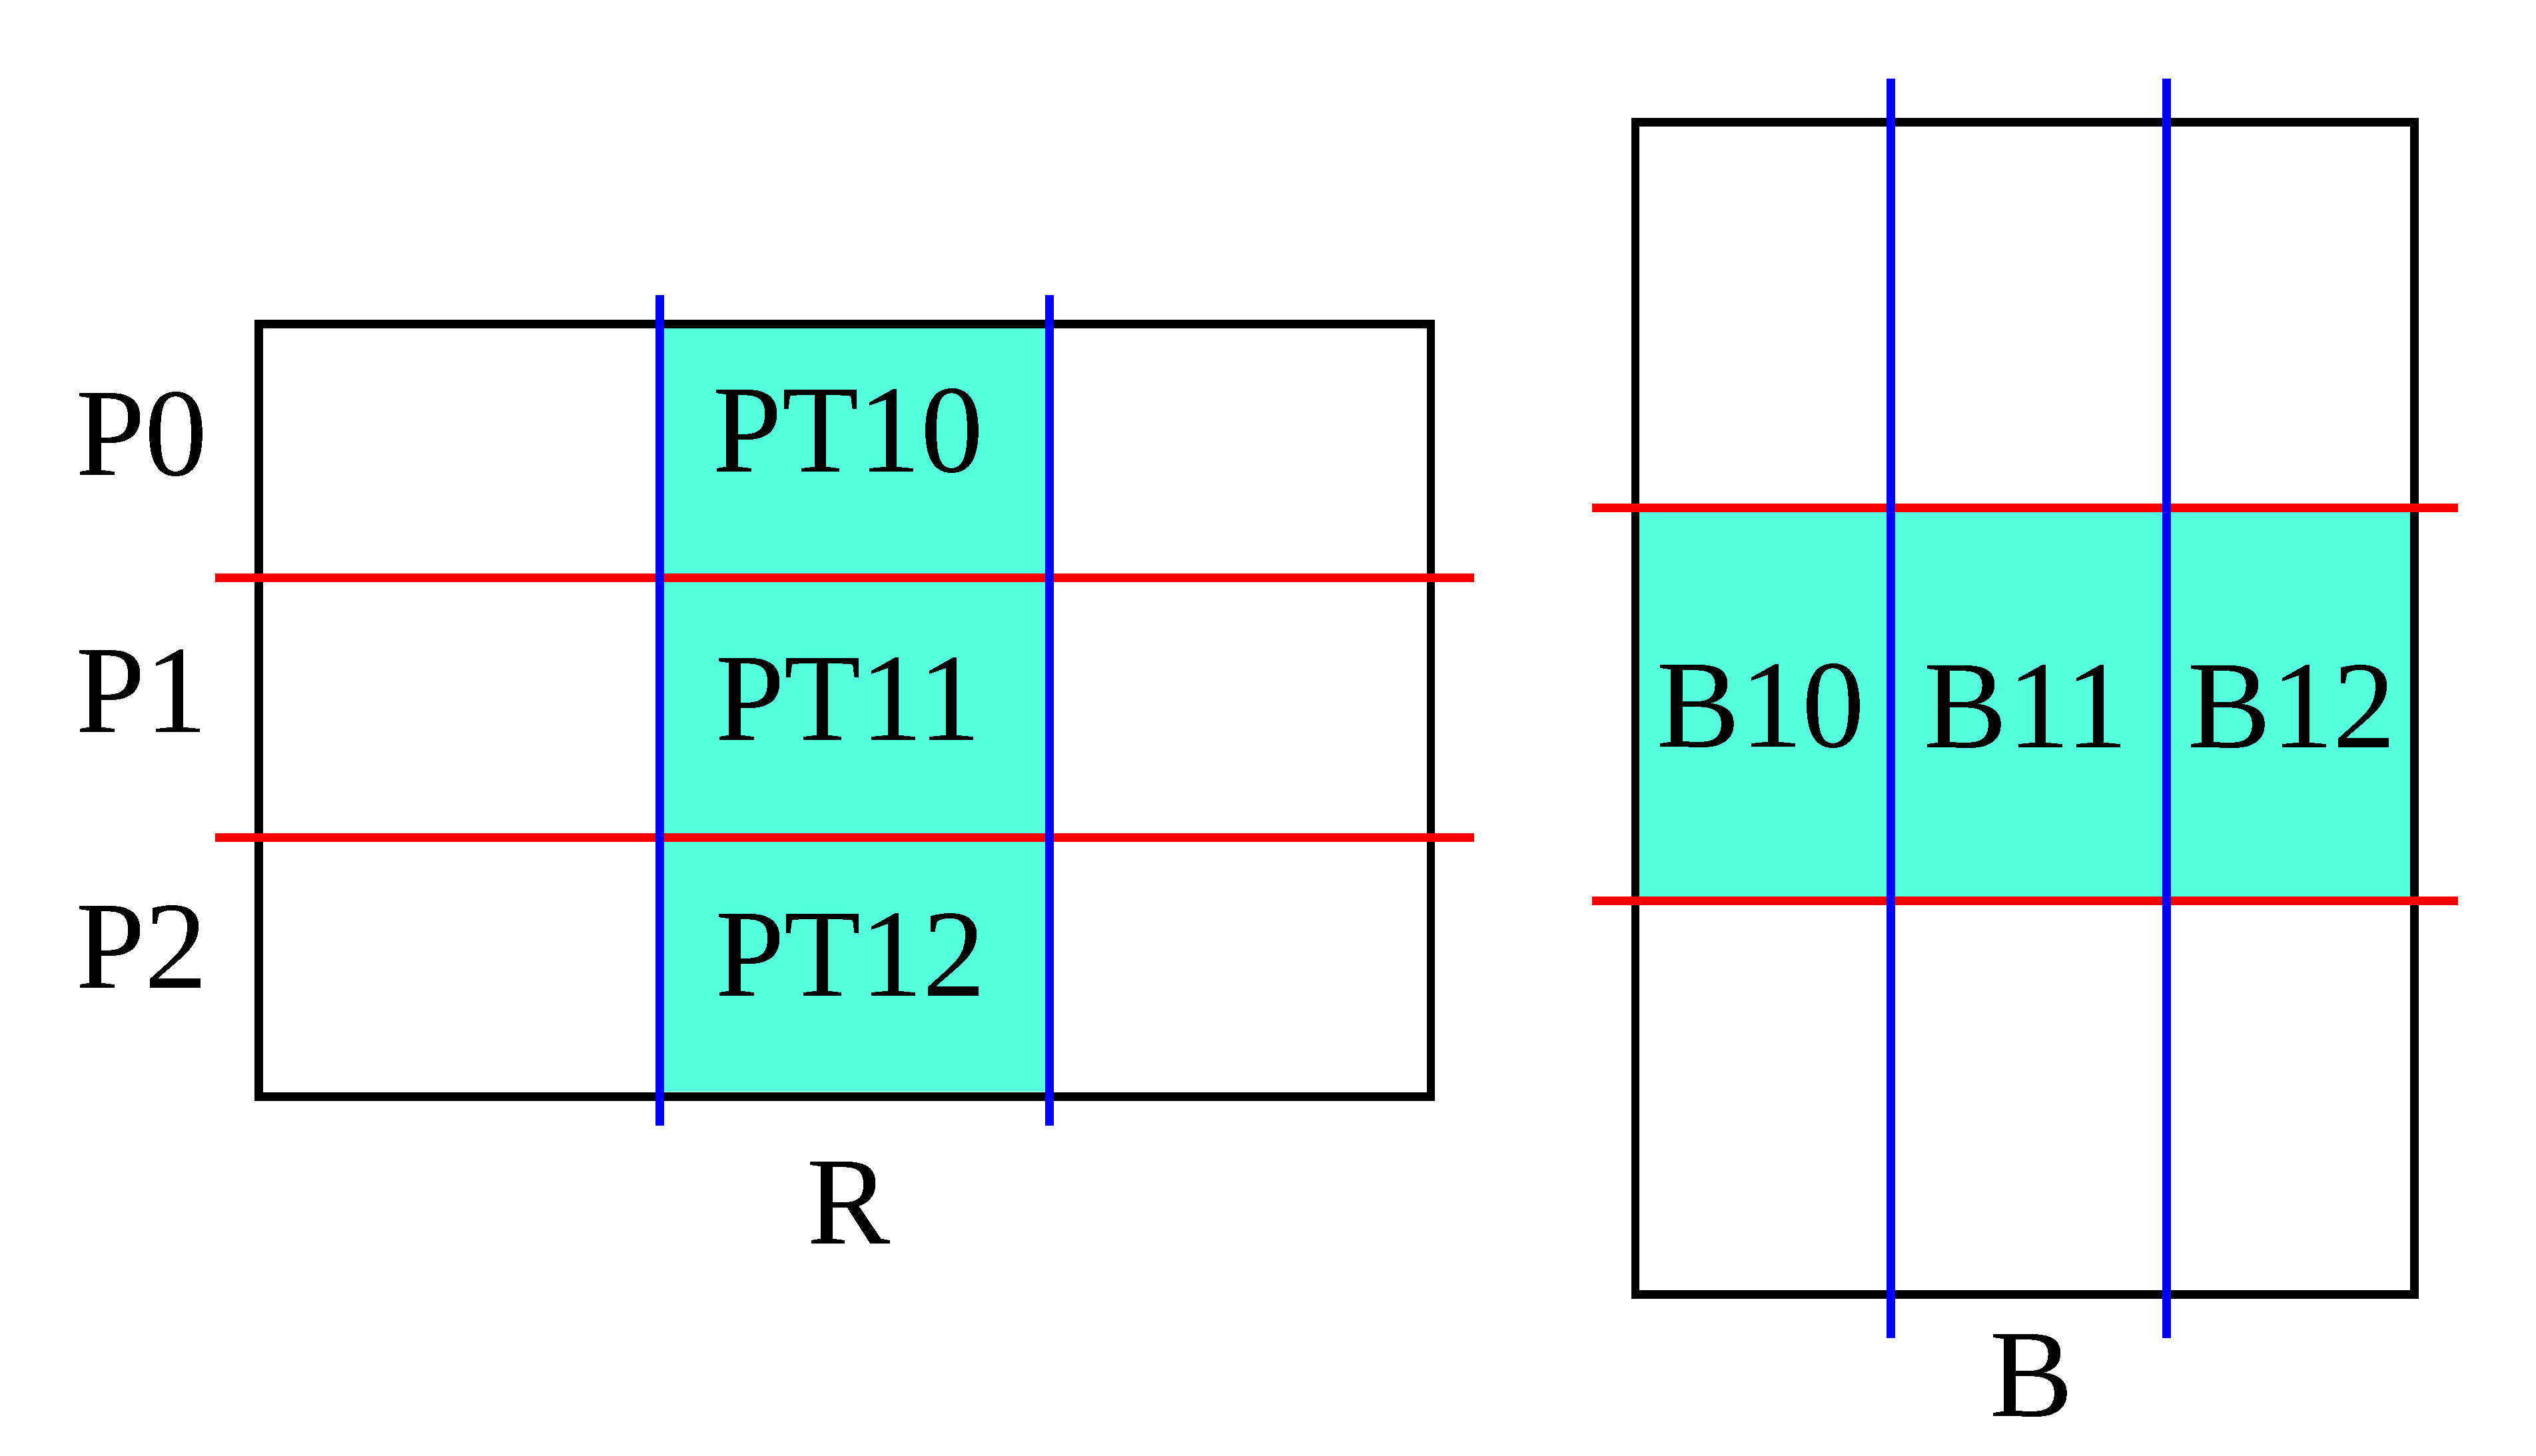
\includegraphics[width=5.5cm,height=3cm]{./figures/part2e.pdf}
 \caption{}
 \label{fig:part2e}
\end{figure}

Using this method, we need to add duplicates twice (explain duplicates). Once, after doing the multplication; Second time, after sorting the result globally and putting the entries on the correct processors. Algorithm~\ref{alg:part2} shows how we have implemented it. Note that each sub-block of $R_i$ should be multiplied by whole $B_i$, in contrary to the naive method, in which each sub-block of $R_i$ is multiplied by only one other sub-block of $B_i$.

\begin{algorithm}[H] 
  %\footnotesize
  \caption{Part 2: $Ac = R \times B$} \label{alg:part2} 
  \begin{algorithmic}[1]
    \Require $P_i$, $B_i$
    \Ensure  $Ac_i$
    \State $PT_i \leftarrow$ compute transpose of $P_i$ (locally)
    \For{$k=0:nprocs$}
      \State $Ac_i \leftarrow\ PT_{ik} \times B_i$
    \EndFor
    \State locally sort $Ac_i$ and add duplicates
    \State globallly sort $Ac_i$ and add duplicates
  \end{algorithmic}
\end{algorithm}


\subsection{Computation}
\label{sec:comp}
Here we assume that the data is available locally, so we discuss it as a serial implementation. We have implemented comptutation in a recursive fashion. We split the matrices recursively in two ways: split by half based on the matrix size, split by half based on number of nonzeros. 

The recursive function, \recmm, includes three cases:
\begin{enumerate}
 \item Case 1: Stop the recursion: perform the multiplication.
 \item Case 2: A is horizontal.
 \item Case 3: A is vertical.
\end{enumerate}

First we explain the first method, splitting based on the matrix sizes.

\subsubsection{Case 1}
\label{sec:case1}
When the stop condition for recursion is satisfied, we will do the multiplication. 
First, we save the result in a dense matrix, then we add the nonzeros to the final matrix. The advantage of using the dense matrix is avoiding a sorting and also adding the duplicates at the end.

\subsubsection{Case 2}
\label{sec:case2}
When A is horizontal, i.e. its row size is less than or equal to its column size, we halve A by column based on its cloumn size (Figure\ref{fig:case2}). Since row size of B eqauls column size of A, we halve B by row, so it will a smiliar split to A, but horizontally.

\begin{figure}[tbh]
 \centering
 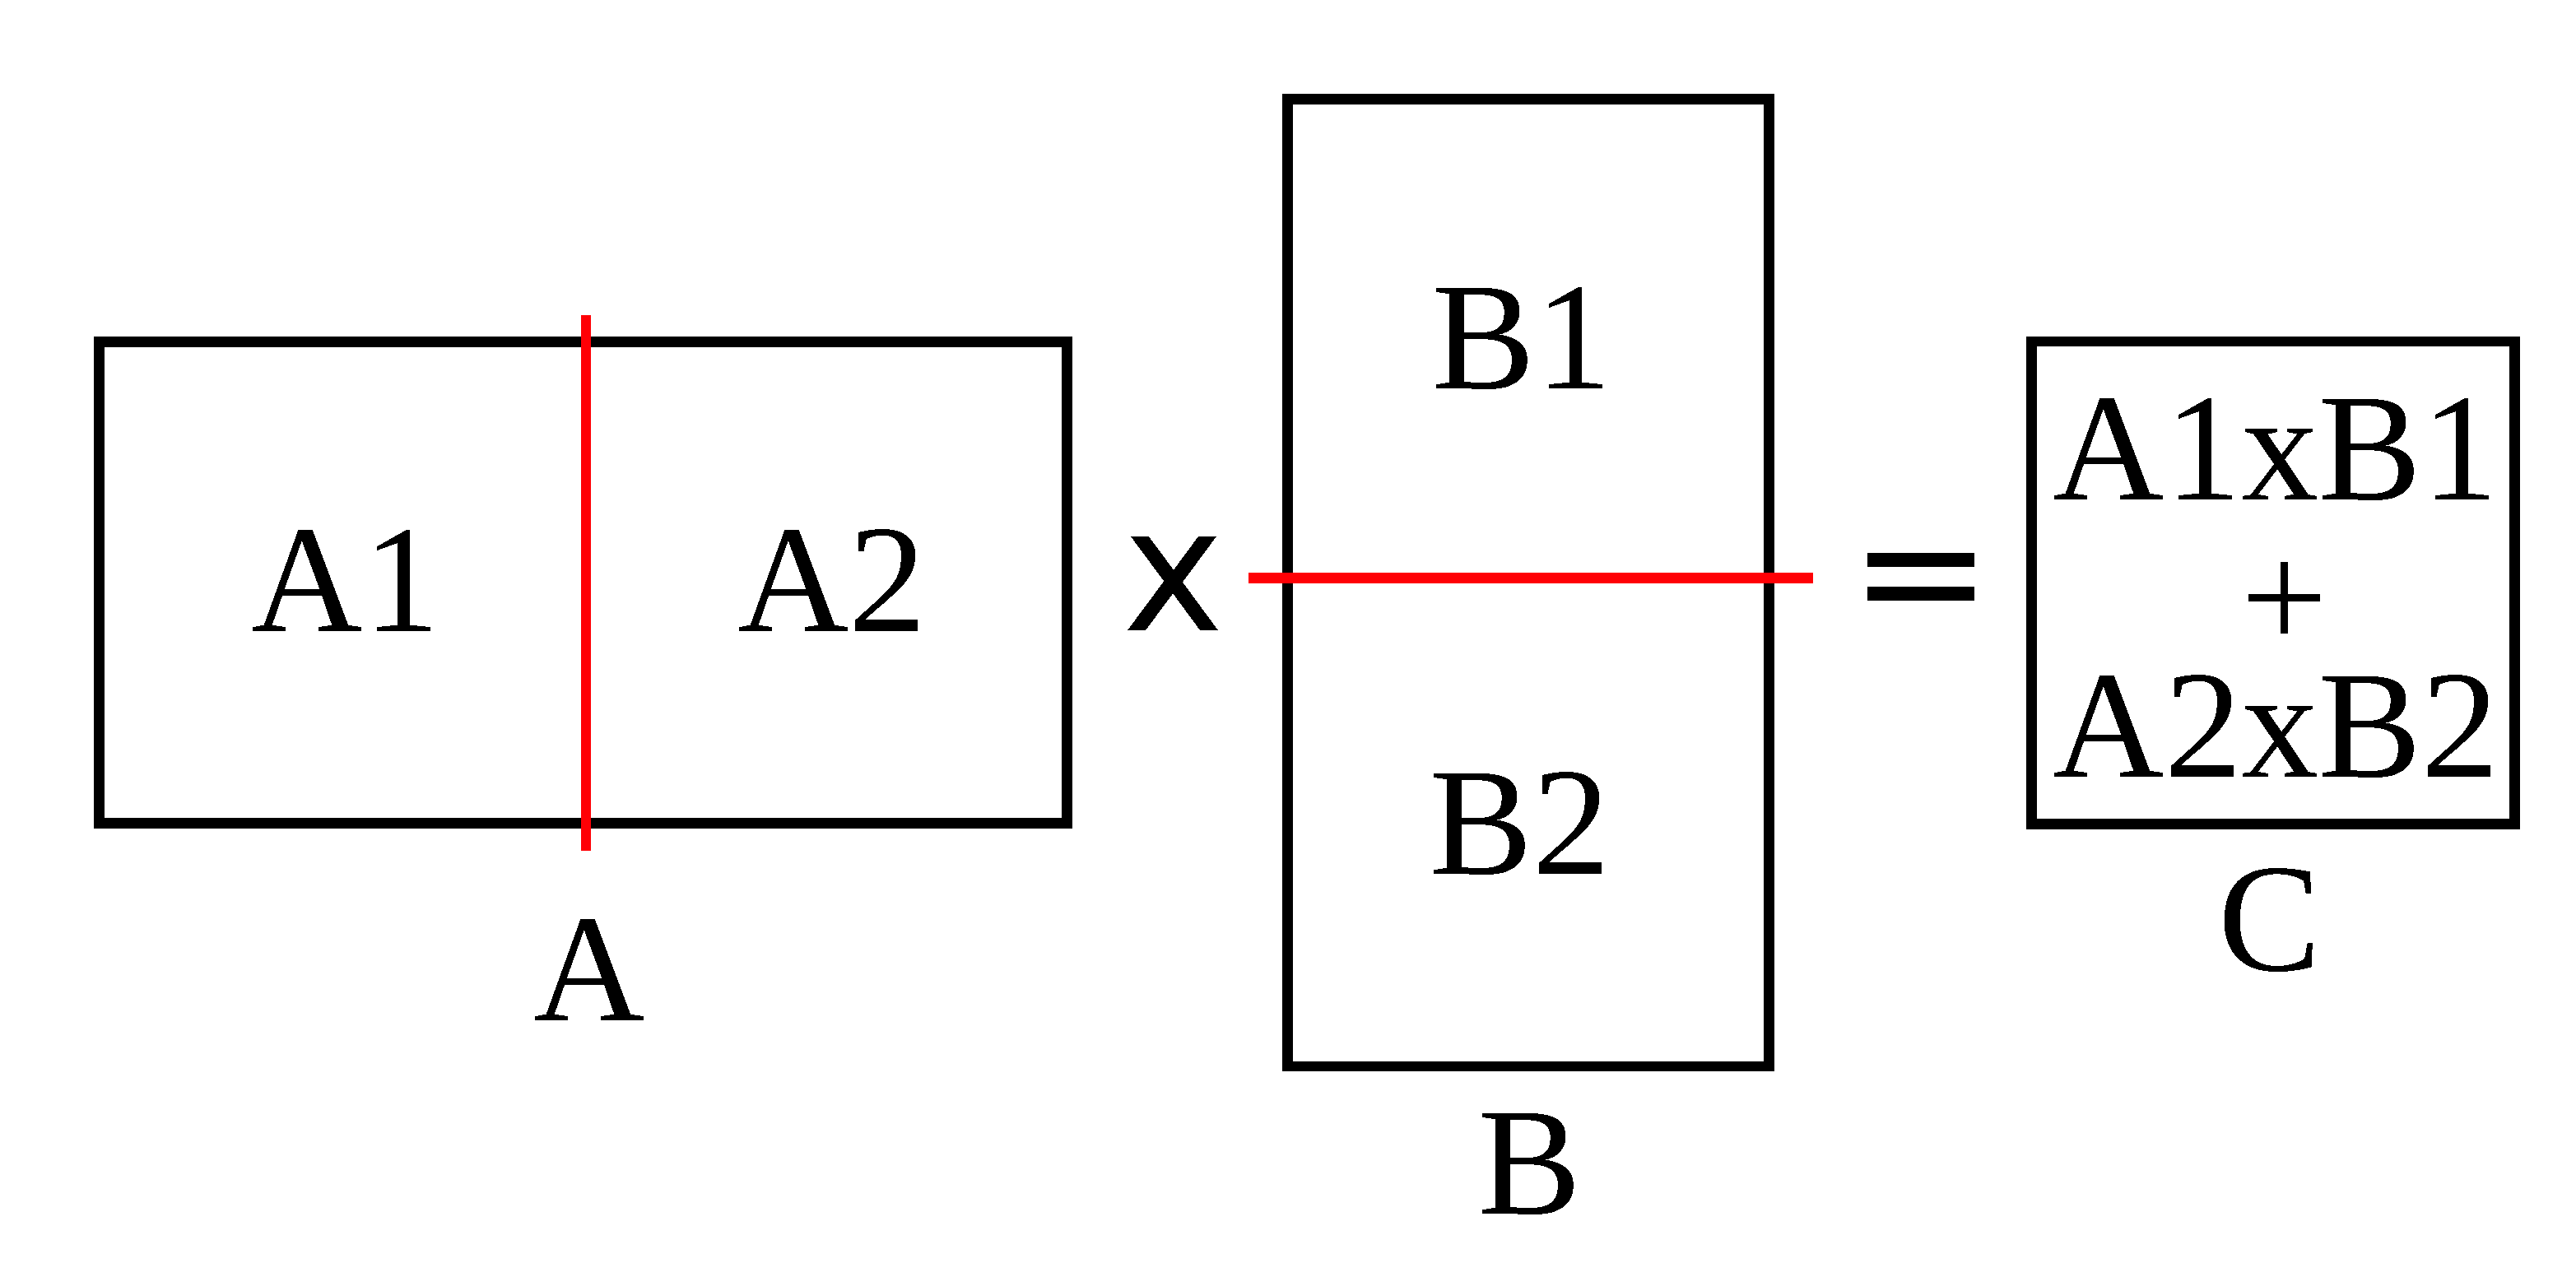
\includegraphics[width=6cm,height=2.7cm]{./figures/case2_001.pdf}
 \caption{}
 \label{fig:case2}
\end{figure}

\begin{algorithm}[H] 
  %\footnotesize
  \caption{Case 2: $C = \recmm2(A, B)$} \label{alg:case2} 
  \begin{algorithmic}[1]
    \Require $A$, $B$
    \Ensure  $C$
    \State $(A1, A2) = \spc(A)$
    \State $(B1, B2) = \spr(B)$
    \State $C1 \leftarrow \recmm(A1,B1)$
    \State $C2 \leftarrow \recmm(A2,B2)$
    \State $C \leftarrow \textsc{mergesort}(C1, C2)$
  \end{algorithmic}
\end{algorithm}

\subsubsection{Case 3}
\label{sec:case3}
When A is vertical, i.e. its row size is greater than its column size, we halve A by row based on its cloumn size and halve B by column (Figure\ref{fig:case3}). In contrary to the previous case, column size of B is not related to row size of A, so they are splitted independently.

\begin{figure}[tbh]
 \centering
 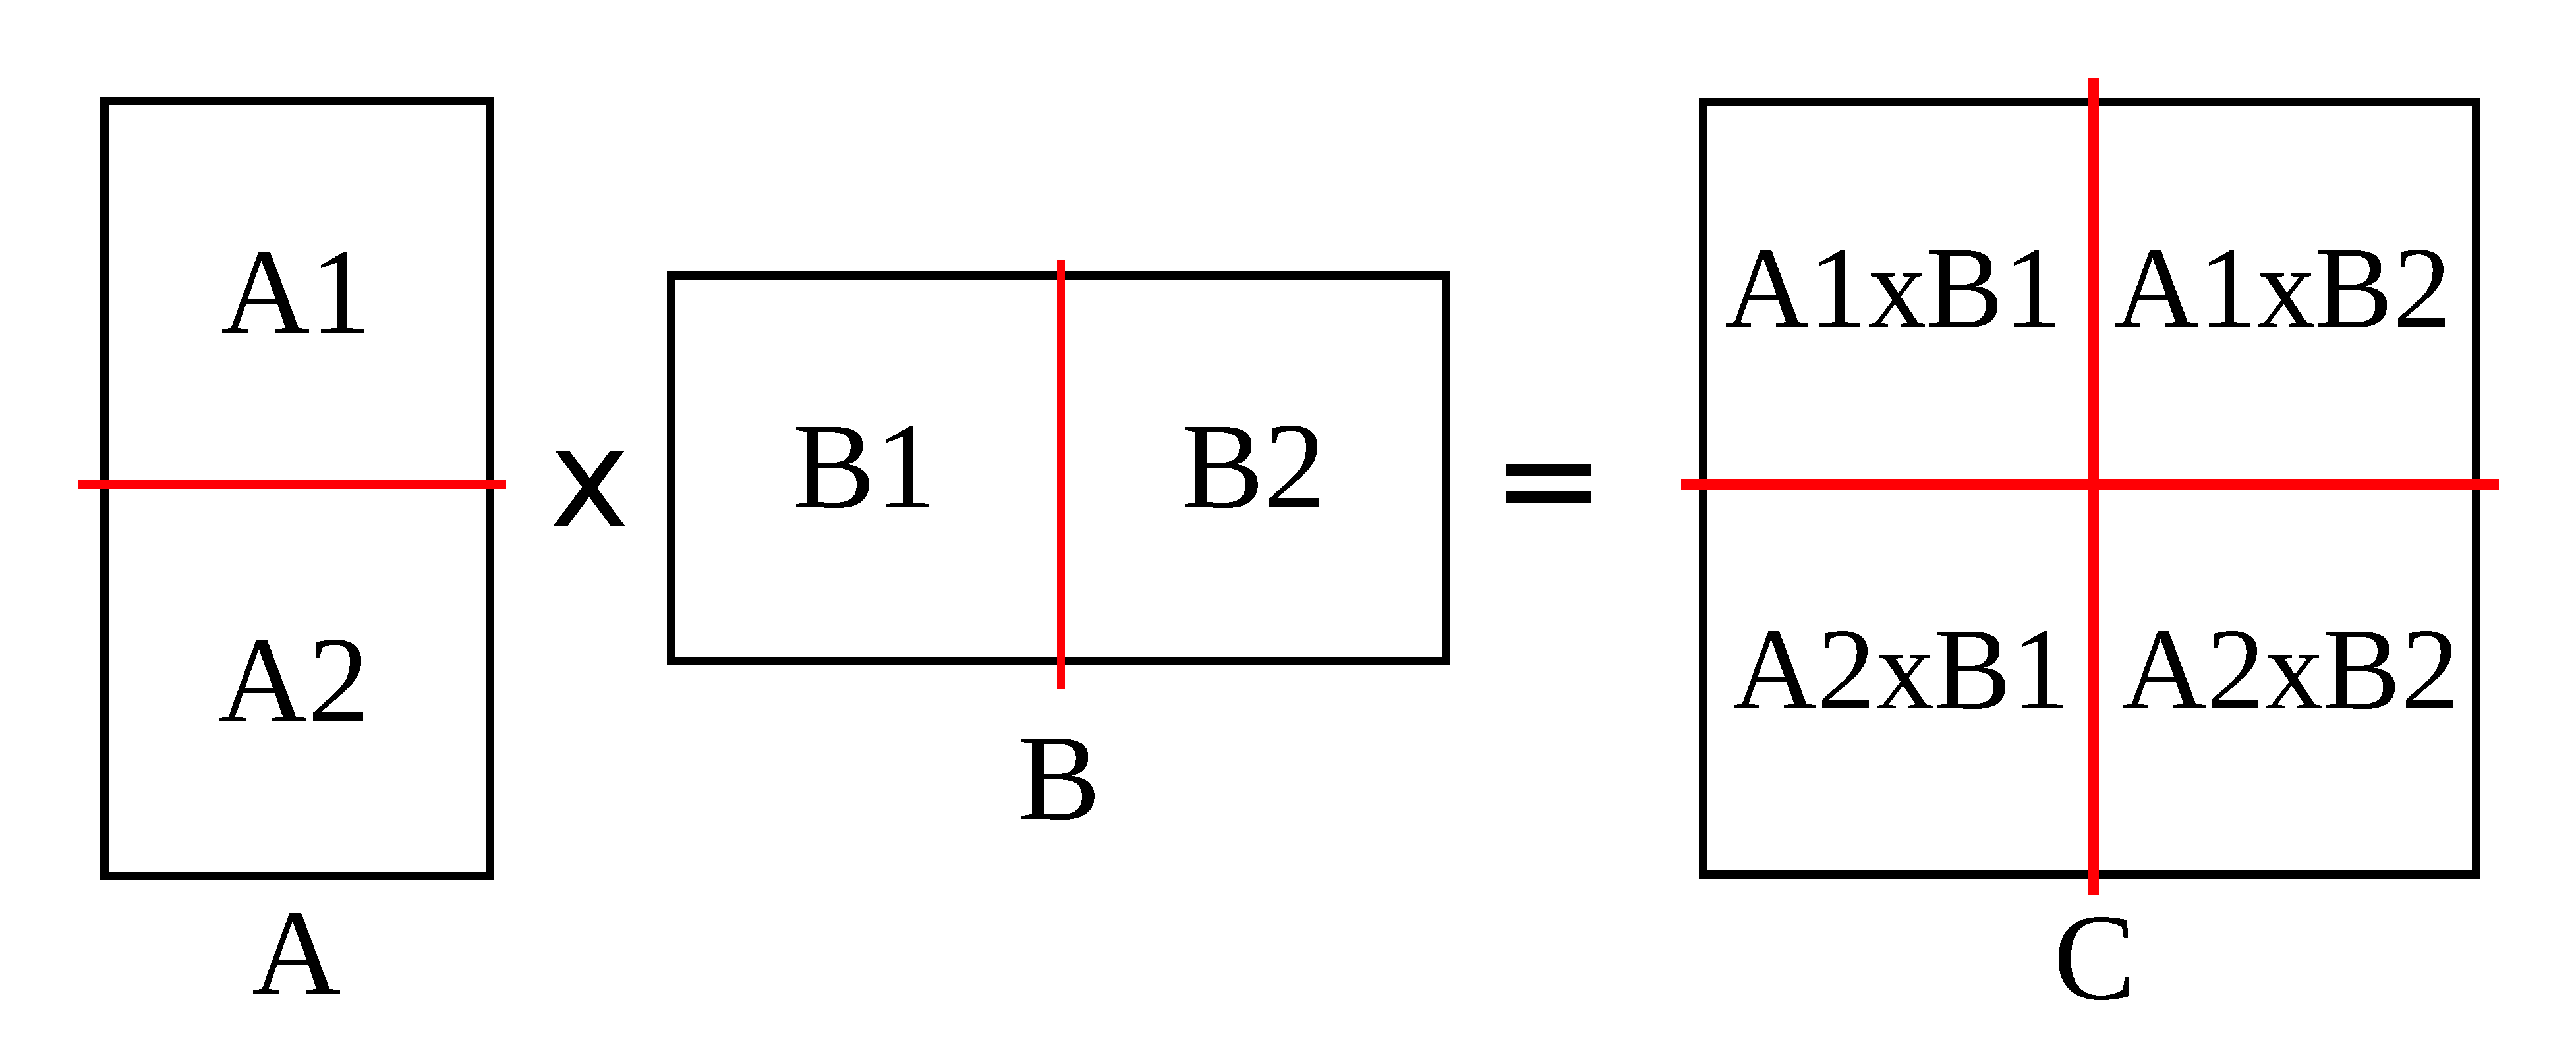
\includegraphics[width=6cm,height=2.7cm]{./figures/case3_001.pdf}
 \caption{}
 \label{fig:case3}
\end{figure}

\begin{algorithm}[H] 
  %\footnotesize
  \caption{Case 3: $C = \recmm3(A, B)$} \label{alg:case3} 
  \begin{algorithmic}[1]
    \Require $A$, $B$
    \Ensure  $C$
    \State $(A1, A2) = \spr(A)$
    \State $(B1, B2) = \spc(B)$
    \State $C \leftarrow \recmm(A1,B1)$
    \State $C \leftarrow \recmm(A2,B1)$
    \State $C \leftarrow \recmm(A1,B2)$
    \State $C \leftarrow \recmm(A2,B2)$
    \State $\textsc{sort}(C)$
  \end{algorithmic}
\end{algorithm}

Explain why we prefer case 2 over case 3, so we have changed condition for case 2 to: when A's row size is less than or equal to \textbf{a multiple of} its column size.

Explain the second method, splitting based on the number of nonzeros.

Swap the computation part with communication, add \recmm ~to communication algos.
